\documentclass{puzz}
\usepackage{tikz}
\usepackage{wrapfig}

\begin{document}

\puzztitle{Puzzle 4: Time-Travel Tour}
\setlength\intextsep{0pt}

\begin{wrapfigure}{r}{0.15\textwidth}
    \centering
    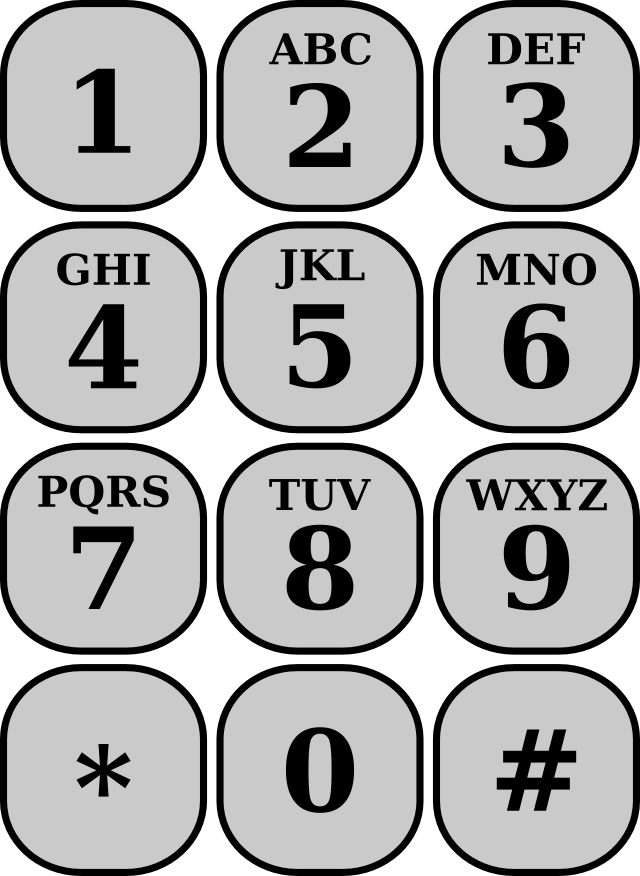
\includegraphics[width=0.15\textwidth]{graphics/keypad}
\end{wrapfigure}

A band of musicians from far away has visited the Mines campus for a tour. They
came with their special \emph{time machine} that lets them teleport around both
space and time by entering destinations using a standard telephone keypad, like
the one shown on the right\footnote{The encoding used to enter these
destinations on the keypad is mysterious. The admissions office has tried
everything from GPS coordinates to UNIX timestamps and has not had any luck.}.

Their tour guide mysteriously went missing after the tour, and the admissions
office wants to find out who the band was to get their tour guide back. They
have recovered the time machine and its most recent travels. Name the band.

\vfill

\begin{tikzpicture}
    \node[label={below:Guggenheim Hall}] (gh) at (0, 0) {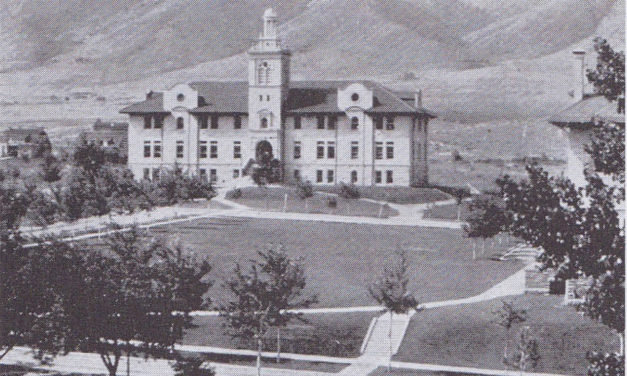
\includegraphics[width=2in]{graphics/gh}};
    \node[label={below:Engineering Hall}] (eh) at (10, 1) {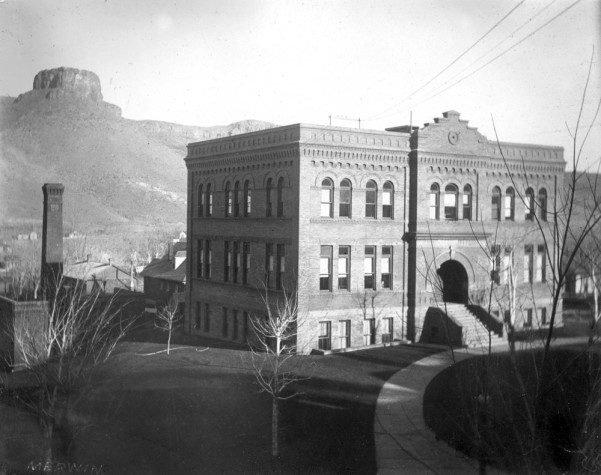
\includegraphics[width=2in]{graphics/eh}};
    \node[label={below:Coolbaugh Hall}] (co) at (12, -5) {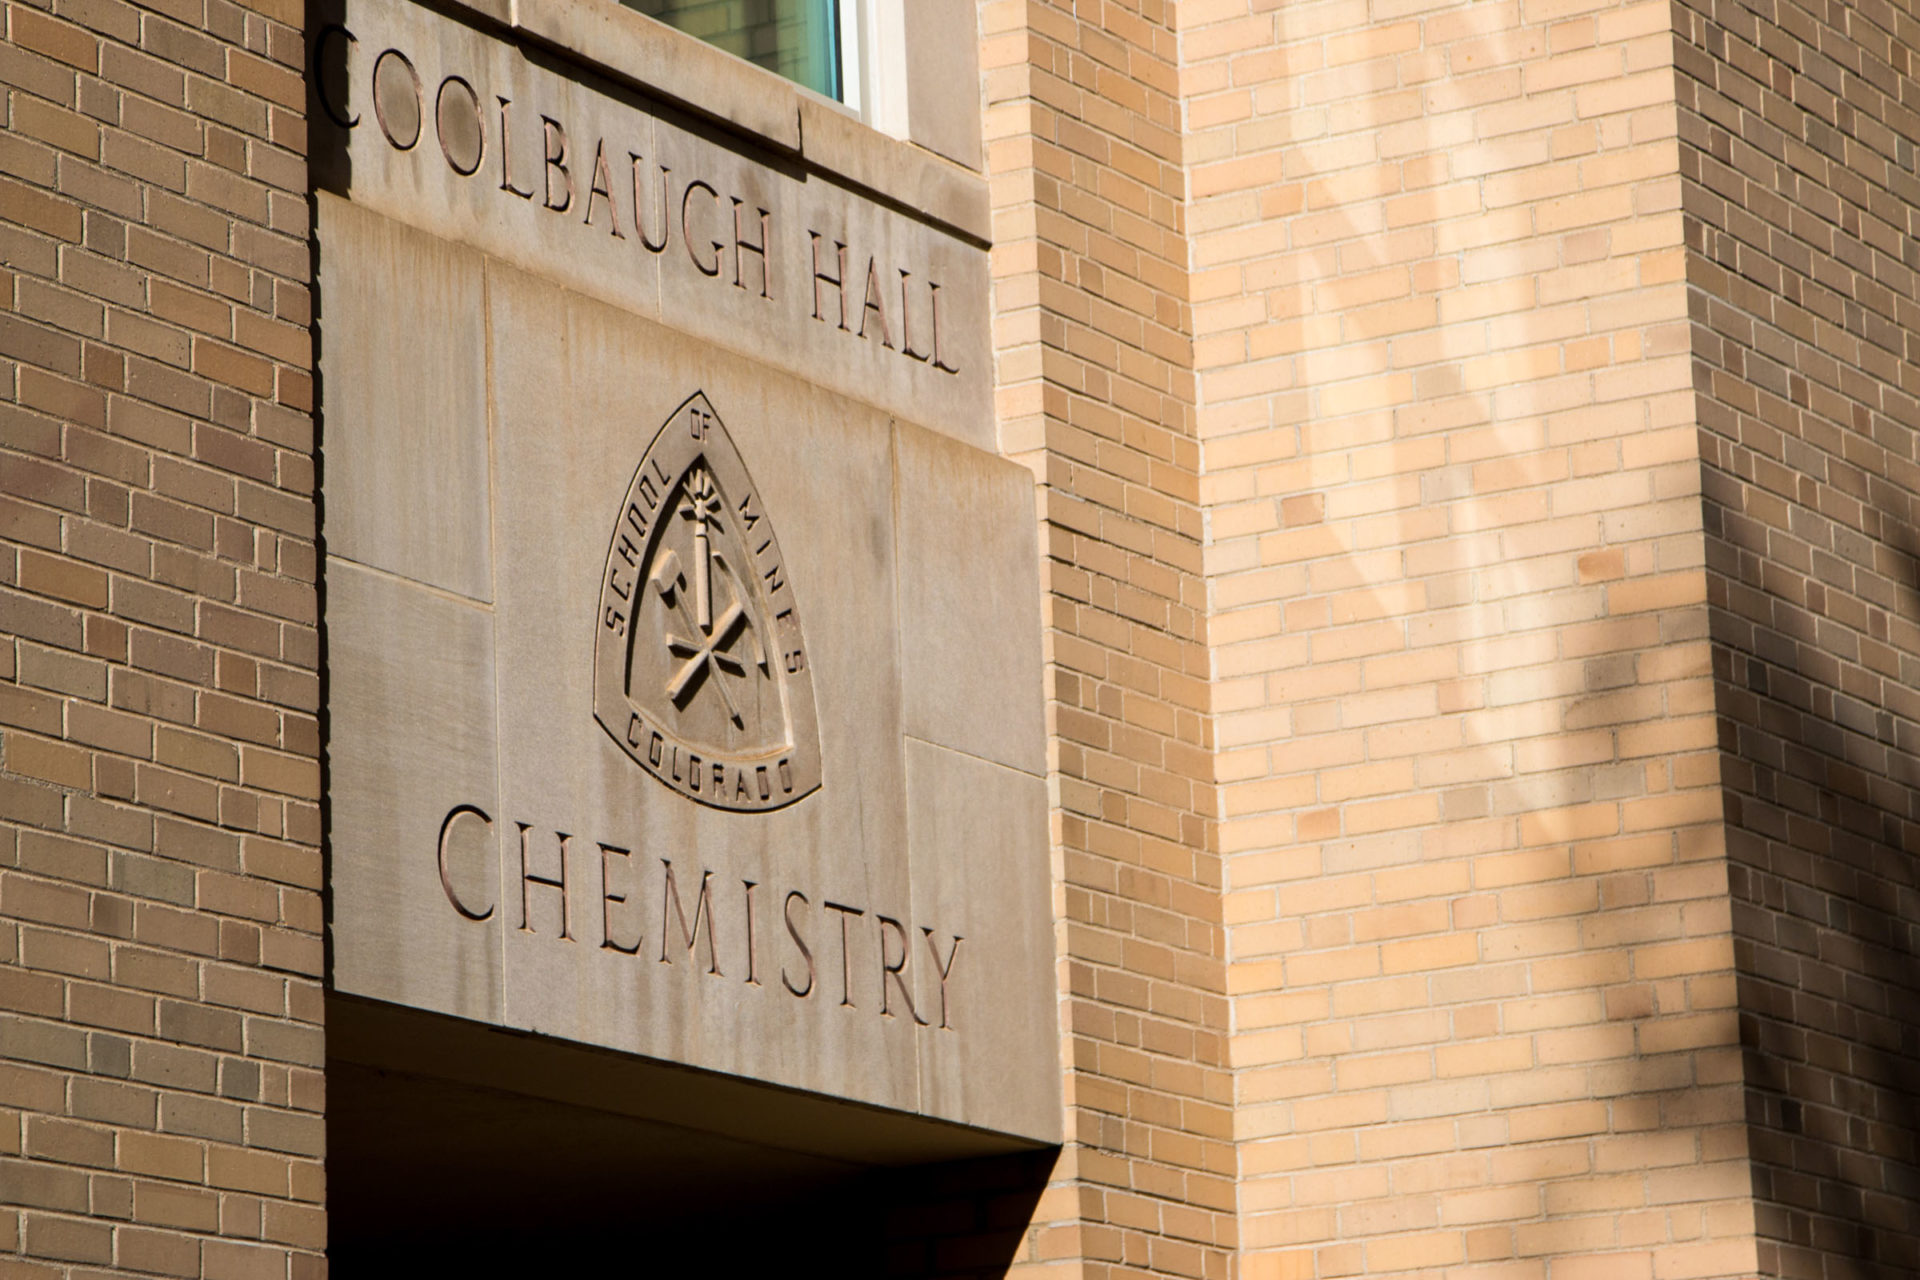
\includegraphics[width=2in]{graphics/co}};
    \node[label={below:Hill Hall}] (hh) at (0.5, -5.5) {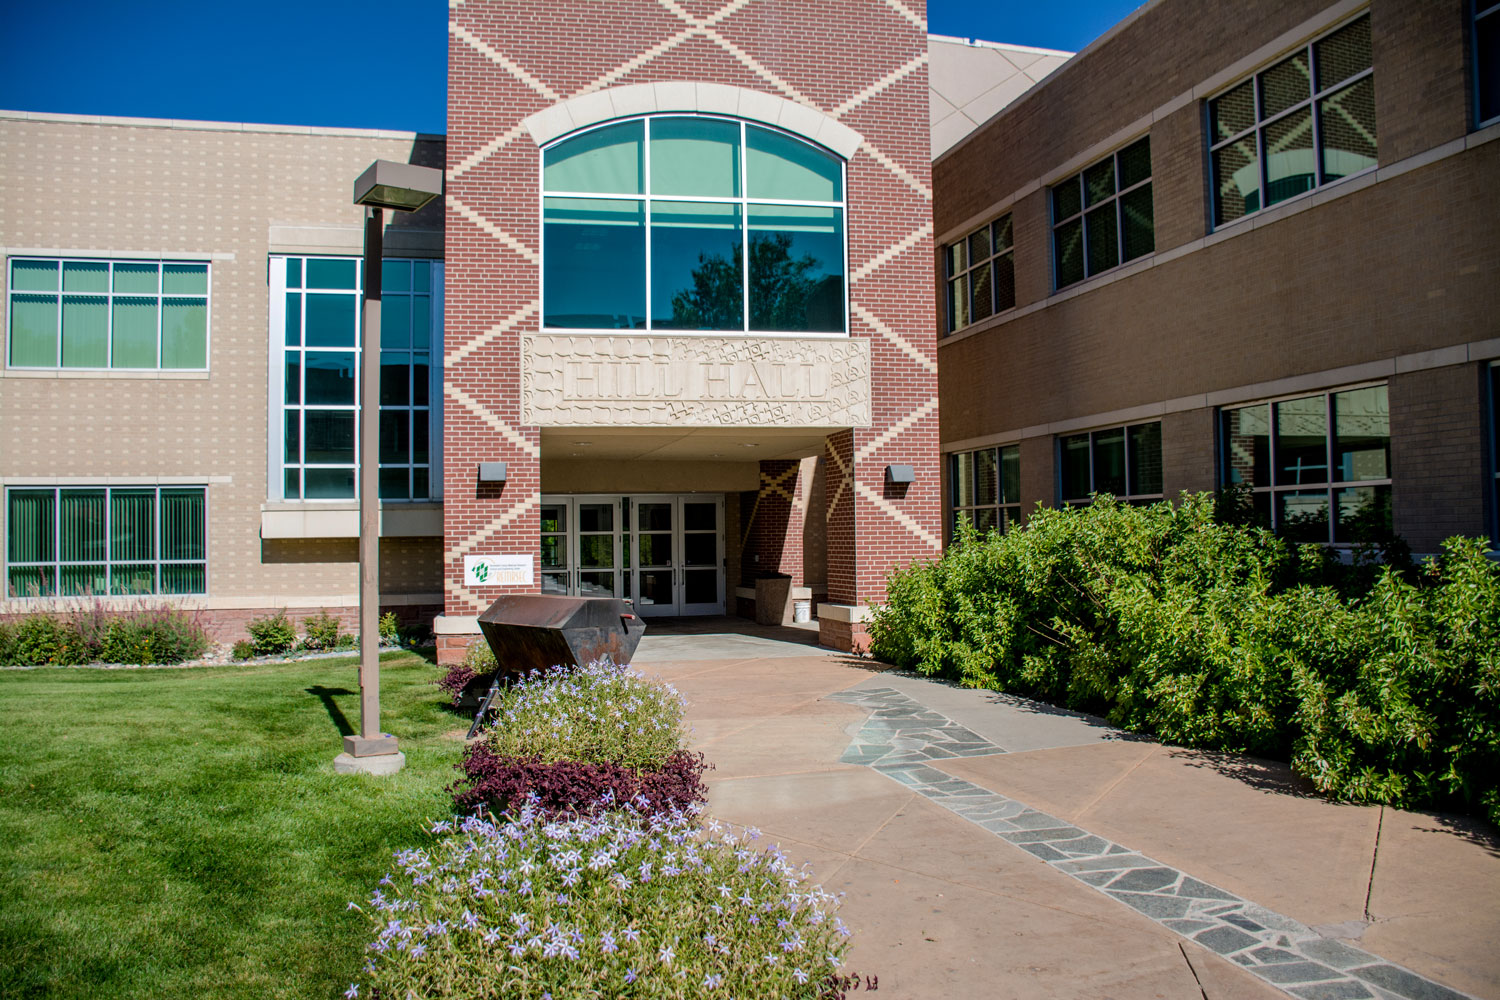
\includegraphics[width=2in]{graphics/hh}};
    \node[label={below:Welcome Center}] (wa) at (6.5, -8) {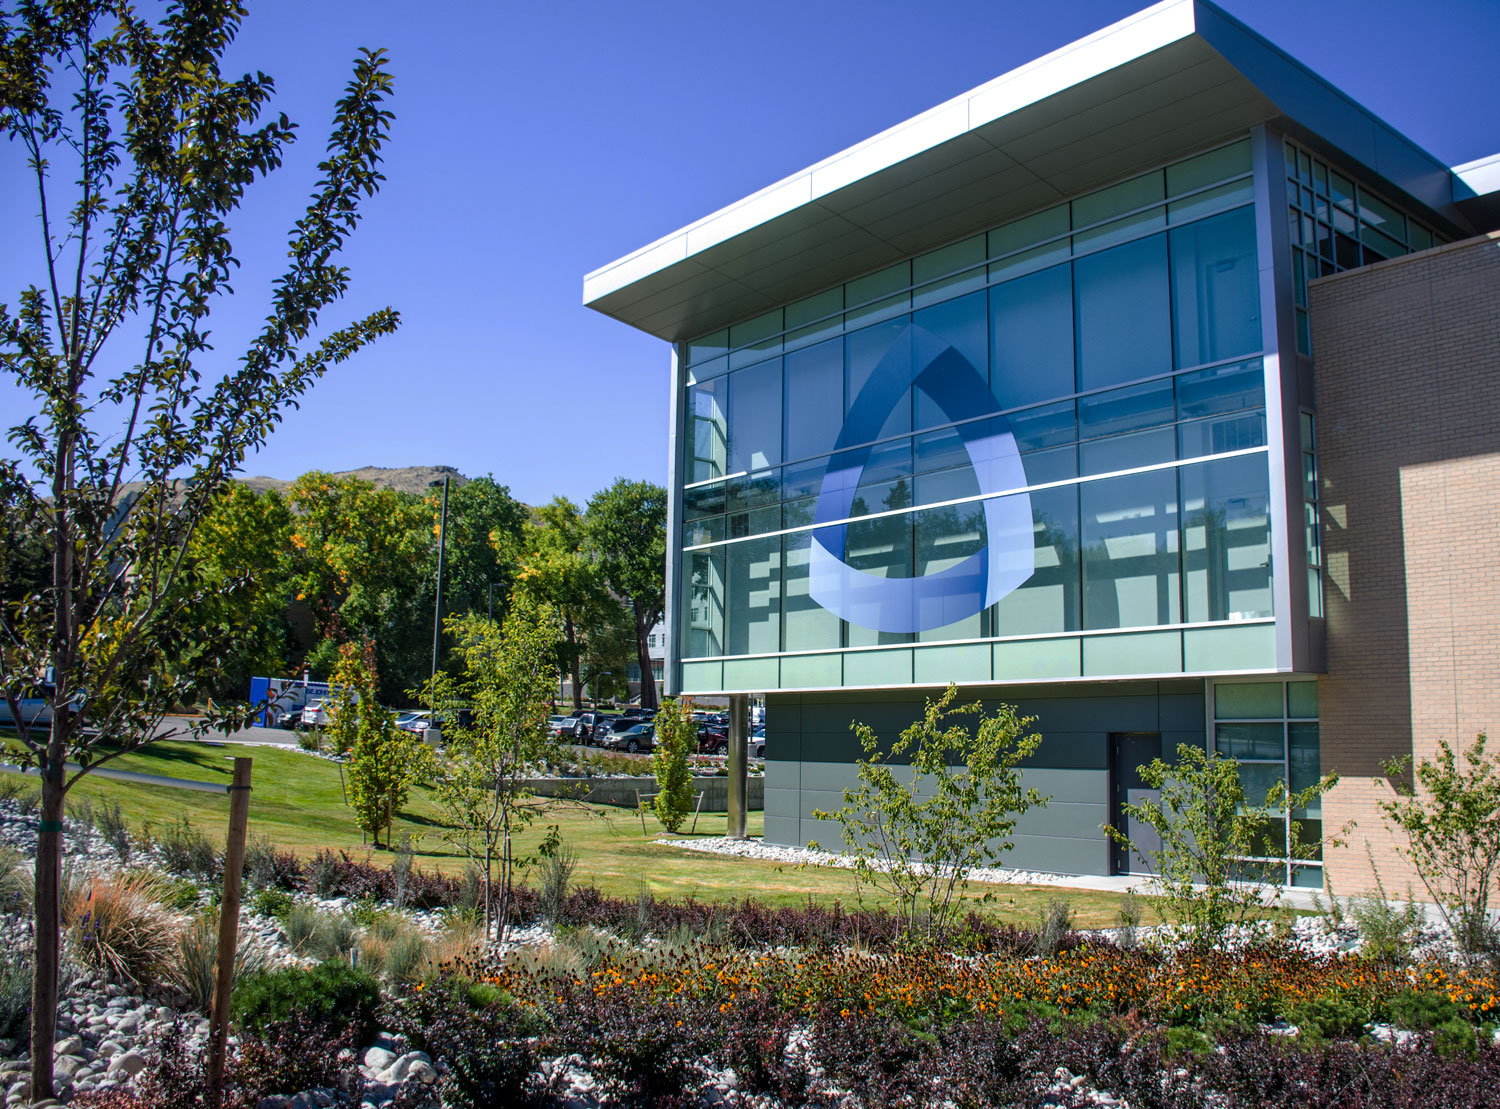
\includegraphics[width=2in]{graphics/wa}};
    \draw[->,ultra thick] (gh) edge[bend left] (eh);
    \draw[->,ultra thick] (eh) edge[bend left] (co);
    \draw[->,ultra thick] (co) edge[bend right] (hh);
    \draw[->,ultra thick] (hh) edge[bend left] (wa);
\end{tikzpicture}

\vfill

\end{document}
